\documentclass[11pt]{amsart}

% Encoding and fonts
\usepackage[T1]{fontenc}
\usepackage[utf8]{inputenc}
\usepackage{lmodern}
\usepackage{microtype}

% Mathematics
\usepackage{amsmath}
\usepackage{amssymb}
\usepackage{amsfonts}
\usepackage{amsthm}
\usepackage{mathtools}

% Layout, figures, and tables
\usepackage{geometry}
\usepackage{enumitem}
\usepackage{booktabs}
\usepackage{array}
\usepackage{tabularx}
\usepackage{graphicx}
\usepackage{placeins}

\geometry{margin=1in}
\emergencystretch=2em

\numberwithin{equation}{section}
\setcounter{tocdepth}{3}
\setcounter{secnumdepth}{3}

% Theorem-like environments
\theoremstyle{plain}
\newtheorem{theorem}{Theorem}[section]
\newtheorem{proposition}[theorem]{Proposition}
\newtheorem{lemma}[theorem]{Lemma}
\newtheorem{corollary}[theorem]{Corollary}
\newtheorem{conjecture}[theorem]{Conjecture}

\theoremstyle{definition}
\newtheorem{definition}[theorem]{Definition}
\newtheorem{experiment}[theorem]{Experiment}
\newtheorem{heuristic}[theorem]{Heuristic}
\newtheorem{question}[theorem]{Question}

\theoremstyle{remark}
\newtheorem{remark}[theorem]{Remark}
\newtheorem{warning}[theorem]{Warning}

\newcommand{\Mertens}{\mathcal M}
\newcommand{\TV}{\mathrm{TV}}
\newcommand{\E}{\mathbb E}
\newcommand{\F}{\mathbb F}
\newcommand{\C}{\mathbb C}
\newcommand{\Z}{\mathbb Z}
\newcommand{\one}{\mathbf 1}
\newcommand{\eps}{\varepsilon}

% Hyperlinks are loaded last.
\usepackage[hidelinks]{hyperref}

\title[Distant square-root audit]{A Distant-Theorem Audit for Pointwise
Square-Root Cancellation in M\"obius Sums}
\author{Research audit prepared for V. Casana}
\date{July 14, 2026}
\hypersetup{
  pdftitle={A Distant-Theorem Audit for Pointwise Square-Root Cancellation in Mobius Sums},
  pdfauthor={Research audit prepared for V. Casana}
}

\begin{document}

\begin{abstract}
We test whether square-root theorems from probability, Boolean analysis,
automatic sequences, frame theory, dynamical systems, empirical-process
theory, discrepancy, random multiplicative chaos, and function fields can be
transferred to the deterministic summatory M\"obius function.  The audit uses
one criterion throughout: an exact representation of the constant vector,
a uniform square-root estimate for every representing kernel, and an inverse
of total-variation or \(\ell^1\) norm \(N^{o(1)}\).  We prove elementary
diagnostic results for positive averaging, random centering, point evaluation
in ambient \(L^p\) spaces, and direct \(\ell^1\) reconstruction.  We also
compute the mean predicted by an unrestricted independent \(p\)-adic surrogate;
it is of order \(N/(\log N)^2\), not of square-root order.  The reported
finite computation on \(455{,}052{,}511\) supplied M\"obius values exhibits a
large mismatch with that surrogate at the final prefix.  None of the theorems
in the audited collection currently supplies the complete transfer criterion
under the exclusions imposed here.  Automatic recursions, function-field
specialization, signed stable sampling, and deterministic transfer operators
are therefore not retained as completed routes in this audit.  A
sign-reversing involution with a square-root exceptional set would imply the
target estimate directly, whereas the one-prime matching graph has an
obstruction of order \(N/\log N\).  Moreover, the exact orthogonal
decomposition of cyclic-window energy contains \(|\Mertens(N)|^2\) as its
constant-mode component.  Thus an uncentered square-root energy estimate
already contains the desired conclusion, while a centered estimate removes
precisely that component.
\end{abstract}

\maketitle
\tableofcontents

\bigskip

\begin{remark}[Status of the document]
\label{rem:document-status}
The statements in theorem-like environments are proved in the text.  Claims
about the literature are cited.  The numerical values in
Section~\ref{sec:numerics} are reported from the supplied computational record;
the underlying binary data and generating script were not part of the present
textual re-audit, so those values are not independently recomputed here.
\end{remark}

\section{Objective and scope}\label{sec:objective}

Let
\begin{equation}\label{eq:mertens-sum}
  \Mertens(N)=\sum_{n\leq N}\mu(n).
\end{equation}
The target scale is
\begin{equation}\label{eq:target}
  |\Mertens(N)|\ll_{\eps}N^{1/2+\eps}
  \qquad (\eps>0).
\end{equation}
This report deliberately avoids using classical character methods, explicit
formulae, zero-density estimates, classical large-sieve arguments, and nilsequence
technology as candidate engines.  Those subjects are already adjacent to the
classical problem.  The purpose is narrower and more severe: locate a theorem
proved for a genuinely different object and determine whether its hypotheses
can be applied to \(\mu\) through an exact and stable representation.

The central conclusion is negative but substantive.  Every route in the
audited collection fails at a named mathematical interface.  In most cases the failure is not
that the available exponent is slightly too weak.  The theorem controls a
fluctuation around an unknown mean, a random input rather than a fixed one, a
coloring that may be chosen rather than the prescribed M\"obius coloring, or
an inverse whose norm destroys the square-root gain.

An earlier version retained frame reconstruction and deterministic transfer
operators as conditional templates.  That classification was too permissive.
Once character estimates, large-sieve methods, zero-density arguments, and
their close analogues are excluded from the search, neither template supplies
an independent mechanism for its required uniform M\"obius correlation bound.
Section~\ref{sec:program} closes both templates and the proposed
sign-reversing-involution reformulation within the declared scope.

\section{The admissibility criterion}\label{sec:criterion}

For each \(N\), let \((\Xi_N,\mathcal A_N)\) be a measurable space and let
\(K_N(n,\xi)\) be a measurable kernel for \(1\leq n\leq N\).  A finite complex
measure \(\nu_N\) on \(\Xi_N\) gives an exact reconstruction when
\begin{equation}\label{eq:exact-reconstruction}
  1=\int_{\Xi_N}K_N(n,\xi)\,d\nu_N(\xi)
  \qquad (1\leq n\leq N).
\end{equation}

\begin{theorem}[Exact stable-transfer lemma]\label{thm:transfer}
Suppose that \eqref{eq:exact-reconstruction} holds and that, for every
\(\eps>0\),
\begin{equation}\label{eq:twisted-bound}
  \sup_{\xi\in\Xi_N}
  \left|\sum_{n\leq N}\mu(n)K_N(n,\xi)\right|
  \leq C_{\eps}N^{1/2+\eps}
\end{equation}
and
\begin{equation}\label{eq:stable-inverse}
  \|\nu_N\|_{\TV}\leq N^{o(1)}.
\end{equation}
Then \eqref{eq:target} holds.
\end{theorem}

\begin{proof}
Finite summation and integration may be interchanged.  Hence
\begin{align}
  \Mertens(N)
  &=\sum_{n\leq N}\mu(n)
    \int_{\Xi_N}K_N(n,\xi)\,d\nu_N(\xi)\notag\\
  &=\int_{\Xi_N}\sum_{n\leq N}\mu(n)K_N(n,\xi)
    \,d\nu_N(\xi).\label{eq:transfer-proof}
\end{align}
Fix \(\eps>0\).  Apply \eqref{eq:twisted-bound} with
\(\eps/2\).  By \eqref{eq:stable-inverse}, for all sufficiently large \(N\),
\(\|\nu_N\|_{\TV}\leq N^{\eps/2}\).  Therefore
\begin{equation}
 |\Mertens(N)|\leq C_{\eps/2}N^{1/2+\eps},
 \label{eq:transfer-final-bound}
\end{equation}
which is \eqref{eq:target}.
\end{proof}

Approximate reconstruction is much less forgiving in the uniform norm.

\begin{proposition}[Cost of reconstruction error]\label{prop:approximation}
Let
\begin{equation}\label{eq:error-vector}
  e_N(n)=1-\int_{\Xi_N}K_N(n,\xi)\,d\nu_N(\xi).
\end{equation}
Under \eqref{eq:twisted-bound},
\begin{equation}\label{eq:error-cost}
  |\Mertens(N)|
  \leq C_{\eps}N^{1/2+\eps}\|\nu_N\|_{\TV}
       +\sqrt N\,\|e_N\|_2.
\end{equation}
In particular, the elementary estimate from a uniform error
\(\|e_N\|_\infty\leq\delta_N\) contributes at most \(N\delta_N\).
\end{proposition}

\begin{proof}
Insert \eqref{eq:error-vector} into \eqref{eq:mertens-sum}.  The integral is
bounded as in Theorem~\ref{thm:transfer}.  Cauchy--Schwarz and
\(\sum_{n\leq N}|\mu(n)|^2\leq N\) give the second term.  The uniform estimate
follows from \(\|e_N\|_2\leq\sqrt N\delta_N\).
\end{proof}

The theorem is elementary, but it prevents a common logical substitution.
An average square-root theorem is useful only after the constant vector has
been reconstructed with a norm that does not consume the gain.

\section{Four universal obstructions}\label{sec:universal}

\subsection{Positive averages cannot hide the constant mode}

\begin{proposition}[Extreme-point obstruction]\label{prop:positive}
Let \(\nu\) be a probability measure and suppose
\(|K(n,\xi)|\leq1\) for all \(n,\xi\).  If
\begin{equation}\label{eq:positive-average}
  1=\int K(n,\xi)\,d\nu(\xi)
\end{equation}
for a fixed \(n\), then \(K(n,\xi)=1\) for \(\nu\)-almost every \(\xi\).
Consequently, an exact positive average of unit-disc oscillatory kernels is
trivial on every reconstructed coordinate.
\end{proposition}

\begin{proof}
The real part satisfies \(\Re K(n,\xi)\leq1\), while its integral is one.
Thus \(\Re K(n,\xi)=1\) almost surely.  The unit-disc condition then forces
\(K(n,\xi)=1\) almost surely.
\end{proof}

Nontrivial reconstruction therefore requires signed or complex weights, or
kernels whose amplitudes exceed one.  Each alternative makes the inverse norm
an essential part of the proof.

\subsection{Randomization controls fluctuations, not the fixed endpoint}

\begin{proposition}[Permutation-centering obstruction]\label{prop:permutation}
Fix real numbers \(a_1,\ldots,a_N\), let \(\Pi\) be a uniformly random
permutation, and put
\begin{equation}\label{eq:permuted-sum}
  S_m(\Pi)=\sum_{j=1}^{m}a_{\Pi(j)},
  \qquad \bar a=N^{-1}\sum_{j=1}^{N}a_j.
\end{equation}
Then
\begin{equation}\label{eq:permutation-mean}
  \E S_m(\Pi)=m\bar a,
  \qquad
  S_N(\Pi)-\E S_N(\Pi)=0
\end{equation}
identically.  Therefore no concentration, central-limit, or strong-approximation
theorem for the centered random process can bound \(\sum_{j=1}^{N}a_j\).
\end{proposition}

\begin{proof}
Every \(a_j\) appears at each position with probability \(1/N\), which gives
the first equality.  Every permutation uses every entry exactly once, so
\(S_N(\Pi)=\sum_j a_j=N\bar a\), proving the second equality.
\end{proof}

For \(a_j=\mu(j)\), the unknown mean is exactly \(\Mertens(N)/N\).  Random
sampling without replacement can estimate that mean if sampled values are
treated as data, but it cannot prove a deterministic upper bound for the
population total from the same population.

\subsection{A random-phase moment bound has no bounded deterministic evaluation}

\begin{proposition}[Ambient point-evaluation obstruction]
\label{prop:evaluation}
Let \((\Omega,\mathcal A,\mathbb P)\) be a probability space and let
\(\omega_0\in\Omega\).  Suppose that there are measurable sets
\(A_k\ni\omega_0\) with \(\mathbb P(A_k)\to0\).  Point evaluation is not
well defined on \(L^p(\Omega)\) equivalence classes.  Moreover, on any linear
space of chosen measurable representatives that contains the normalized
indicators below, every linear functional agreeing with evaluation at
\(\omega_0\) is unbounded with respect to the ambient \(L^p\) norm, for
\(1\leq p<\infty\).
\end{proposition}

\begin{proof}
Take
\begin{equation}
 f_k=\mathbb P(A_k)^{-1/p}\one_{A_k}.
 \label{eq:point-evaluation-test-functions}
\end{equation}
Then \(\|f_k\|_p=1\), whereas
\(|f_k(\omega_0)|=\mathbb P(A_k)^{-1/p}\to\infty\).  Thus no such evaluation
functional is bounded in the ambient \(L^p\) norm.  The preliminary statement
follows because changing a representative on a null set can change its value
at \(\omega_0\).
\end{proof}

\begin{remark}
\label{rem:restricted-evaluation}
Proposition~\ref{prop:evaluation} is an ambient-space statement.  It does not
exclude a bounded evaluation theorem on a smaller regularity class, such as a
finite-dimensional polynomial space equipped with a stronger norm.  A
transfer argument based on random phases would need precisely such a
restricted theorem, with constants uniform in the arithmetic parameters.
\end{remark}

\begin{corollary}[Exact loss on a finite Rademacher cube]
\label{cor:rademacher-evaluation}
Let \(\Omega_m=\{-1,1\}^m\) carry the uniform probability measure, fix
\(\omega_0\in\Omega_m\), and let
\(E_{\omega_0}f=f(\omega_0)\).  For every \(1\leq p<\infty\),
\begin{equation}\label{eq:rademacher-evaluation-norm}
  \|E_{\omega_0}\|_{L^p(\Omega_m)\to\mathbb C}=2^{m/p}.
\end{equation}
In particular, passing from an \(L^2\) average over \(m\) Rademacher prime
phases to one prescribed configuration has optimal worst-case loss
\(2^{m/2}\).
\end{corollary}

\begin{proof}
For every \(f:\Omega_m\to\mathbb C\),
\begin{equation}\label{eq:rademacher-upper}
  \|f\|_p^p
  =2^{-m}\sum_{\omega\in\Omega_m}|f(\omega)|^p
  \geq 2^{-m}|f(\omega_0)|^p.
\end{equation}
Thus \(|E_{\omega_0}f|\leq2^{m/p}\|f\|_p\).  Equality holds for every
nonzero function supported on the singleton \(\{\omega_0\}\), proving
\eqref{eq:rademacher-evaluation-norm}.
\end{proof}

For the unrestricted space of all functions on the prime-sign cube with one
coordinate for every \(p\leq N\), one has \(m=\pi(N)\), so the ambient
worst-case norm is \(2^{\pi(N)/2}\).  This is not \(N^{o(1)}\), since the
prime number theorem gives \(\pi(N)\sim N/\log N\)
\cite{MontgomeryVaughan2007}.  The statement is not a
claim that this ambient norm is sharp on every restricted arithmetic
polynomial subspace.

\subsection{Hilbert-space stability is not the required stability}

\begin{proposition}[The \(\ell^1\) reconstruction cost]\label{prop:frame}
Let \(u_1,\ldots,u_m\in\mathbb C^N\), let
\(\one_N=\sum_{j=1}^{m}c_ju_j\), and suppose
\(\|u_j\|_2\leq L\).  Then
\begin{equation}\label{eq:l1-lower}
  \|c\|_1\geq\frac{\sqrt N}{L}.
\end{equation}
Moreover, if \(|\langle a,u_j\rangle|\leq B\) for all \(j\), the direct
reconstruction argument yields only
\begin{equation}\label{eq:frame-transfer}
  |\langle a,\one_N\rangle|\leq B\|c\|_1.
\end{equation}
An \(\ell^2\) inverse bound does not replace the \(\ell^1\) quantity in
\eqref{eq:frame-transfer}.
\end{proposition}

\begin{proof}
The triangle inequality gives
\(
 \sqrt N=\|\one_N\|_2\leq\sum_j|c_j|\|u_j\|_2\leq L\|c\|_1.
\)
The second assertion follows by pairing the reconstruction with \(a\) and
using the triangle inequality.
\end{proof}

Kashin representations and restricted-invertibility theorems are powerful
\(\ell^2\) stability results.  They do not, by themselves, supply the
\(\ell^1\) coefficient bound used in the direct triangle-inequality argument
\eqref{eq:frame-transfer}.  An \(\ell^2\) reconstruction could still be useful
if accompanied by a matching \(\ell^2\) estimate for the correlation vector;
no such estimate is obtained from Proposition~\ref{prop:frame}.

\section{Martingales and exchangeable pairs}\label{sec:martingales}

Gordin's method and its successors transfer central-limit and invariance
principles from martingale differences to stationary processes
\cite{Gordin1969,GordinPeligrad2011,PeligradUtev2005}.  Chatterjee's
exchangeable-pair method derives concentration from an antisymmetric coupling
and a regression structure \cite{Chatterjee2007}.  These are genuine
square-root theories, but their centering is structural rather than cosmetic.

\begin{proposition}[Constant inputs have zero martingale differences]
\label{prop:doob}
Regard each deterministic number \(a_n\) as a constant random variable on a
probability space, adapted to any filtration.  Then
\begin{equation}\label{eq:deterministic-doob}
  a_n-\E(a_n\mid\mathcal F_{n-1})=0.
\end{equation}
Hence the canonical martingale-difference part of this constant-random-variable
encoding is zero.
\end{proposition}

\begin{proof}
A constant random variable is measurable with respect to every sigma-field and
its conditional expectation equals the same constant.
\end{proof}

Randomly permuting the sequence creates nonzero intermediate fluctuations, but
Proposition~\ref{prop:permutation} shows that the endpoint fluctuation is still
zero.  Multiplying the fixed values by independent mean-zero signs creates a
martingale-difference model under the natural filtration, but changes \(\mu\)
into a different object.  An exchangeable prime-factor move would be relevant
only after proving a regression identity whose remainder is small uniformly
at the fixed M\"obius configuration.  No such identity is supplied by the
exchangeable-pair theorem; it would be the new arithmetic input.

The Maxwell--Woodroofe condition used by Peligrad and Utev contains norms of
conditional expectations of partial sums.  For a proposed deterministic
encoding of M\"obius, verifying those conditional expectations at the required
scale is not automatic and may contain the original cancellation problem.
The route is therefore conditional, not an application of an existing theorem.

\section{Boolean hypercontractivity and prime divisibility}\label{sec:boolean}

For a squarefree integer,
\begin{equation}\label{eq:boolean-parity}
  \mu(n)=(-1)^{\sum_{p\leq N}\one_{p\mid n}}.
\end{equation}
This resembles a Walsh character on a prime-divisibility cube.  Bonami--Beckner
hypercontractivity controls polynomial norms on product spaces
\cite{Bonami1970,Beckner1975}.  The resemblance fails in two independent ways:
the observable is a high-degree parity character, and the divisibility vectors
of integers in an interval are not independent at the resolution needed for
that parity.

The unrestricted independent \(p\)-adic surrogate makes the discrepancy
quantitative.  It is not the factorization law of an integer chosen uniformly
from \([1,N]\); it deliberately discards the global size constraint.  Let
\((V_p)_p\) be independent with
\begin{equation}\label{eq:padic-model}
  \mathbb P(V_p=j)=(1-p^{-1})p^{-j},\qquad j\geq0,
\end{equation}
and extend \(\mu(p^{V_p})\) multiplicatively.

\begin{theorem}[Mean of the independent \(p\)-adic surrogate]\label{thm:boolean-mismatch}
For the model \eqref{eq:padic-model},
\begin{equation}\label{eq:local-expectation}
  \E\mu(p^{V_p})=(1-p^{-1})^2
\end{equation}
and therefore
\begin{equation}\label{eq:global-model-mean}
  \E\prod_{p\leq N}\mu(p^{V_p})
  =\prod_{p\leq N}(1-p^{-1})^2
  \sim \frac{e^{-2\gamma}}{(\log N)^2}.
\end{equation}
Consequently, an independent-prime population of \(N\) observations has mean
of order \(N/(\log N)^2\), which exceeds \(N^{1/2+\eps}\) for every fixed
\(\eps<1/2\) and all sufficiently large \(N\).
\end{theorem}

\begin{proof}
Only \(V_p=0\) and \(V_p=1\) contribute.  Hence
\begin{align}
 \E\mu(p^{V_p})
 &=\mathbb P(V_p=0)-\mathbb P(V_p=1)\notag\\
 &=(1-p^{-1})-(p^{-1}-p^{-2})=(1-p^{-1})^2.
 \label{eq:local-proof}
\end{align}
Independence gives the product.  Mertens' product theorem yields the
asymptotic in \eqref{eq:global-model-mean}; see
\cite{MontgomeryVaughan2007}.  Finally,
\(N^{1/2-\eps}/(\log N)^2\to\infty\).
\end{proof}

Thus the unrestricted product surrogate does not reproduce the mean behavior
of the finite integer prefixes.  This diagnoses the loss caused by discarding
the global size and divisibility constraints.  It does not prove that every
Boolean-analytic formulation must fail; a relevant theorem would have to
retain those arithmetic constraints and control the high-degree parity
observable without replacing it by the independent surrogate.

\section{Automatic sequences and exact recursions}\label{sec:automatic}

The Rudin--Shapiro construction gives deterministic signs with square-root
Fourier growth through an exact two-channel recursion \cite{Rudin1959}.  This is
one of the cleanest distant examples of deterministic square-root cancellation.
It does not transfer by multiplication.

\begin{proposition}[Untwisting obstruction]\label{prop:untwist}
Let \(r(n)\in\{-1,1\}\) be any fixed sequence and define
\(b(n)=\mu(n)r(n)\).  The identity
\begin{equation}\label{eq:untwist}
  \Mertens(N)=\sum_{n\leq N}b(n)r(n)
\end{equation}
is exact.  More generally, within the class of sign sequences, bounds
\(\sum_{n\leq N}b(n)=O(\sqrt N)\) and
\(\sum_{n\leq N}r(n)=O(\sqrt N)\) do not imply a square-root bound for
\(\sum_{n\leq N}b(n)r(n)\).
\end{proposition}

\begin{proof}
The identity follows from \(r(n)^2=1\).  For the general non-implication, take
\(b(n)=r(n)\), with \(r\) equal to a Rudin--Shapiro sign sequence.  Both
unweighted sums are then \(O(\sqrt N)\), whereas
\(\sum_{n\leq N}b(n)r(n)=N\).
\end{proof}

M\"ullner proved qualitative M\"obius orthogonality for all automatic
sequences \cite{Muellner2017}.  This important theorem estimates
\(\sum\mu(n)r(n)=o(N)\); it does not provide the uniform square-root estimate
and stable family reconstruction in Theorem~\ref{thm:transfer}.  The exact
Rudin--Shapiro recursion is therefore a model of the desired phenomenon, not a
known engine for the constant mode.

\section{Frames, restricted inverses, and discrepancy}\label{sec:frames}

Restricted invertibility, Kashin representations, and Kadison--Singer paving
give strong stability and partition theorems
\cite{LyubarskiiVershynin2010,NaorYoussef2017,MSS2015}.  Spencer's discrepancy
theorem constructs a signing with discrepancy of square-root order
\cite{Spencer1985}.  These results solve different quantifier problems.

A fixed frame satisfying frame bounds gives stable \(\ell^2\)
reconstruction for vectors in its span.  Discrepancy theory states that, for
suitable set systems, there exists a favorable coloring.  The M\"obius problem
instead presents one prescribed coloring and asks for its correlation with one
fixed vector.  Neither existence theorem makes that coloring selectable.

Proposition~\ref{prop:frame} identifies the norm that matters.  In a unit-norm
orthonormal basis every representation of \(\one_N\) has coefficient
\(\ell^2\)-norm \(\sqrt N\) and hence \(\ell^1\)-norm at least \(\sqrt N\).
For the Fourier basis the constant mode is a single coefficient, so a uniform
bound that includes it already contains the desired estimate.  Redundancy may
improve robustness, but no theorem in the audited collection simultaneously
supplies
\begin{equation}\label{eq:frame-needed}
  \one_N=\sum_jc_ju_j,\qquad
  \|c\|_1=N^{o(1)},\qquad
  \sup_j|\langle\mu,u_j\rangle|\ll N^{1/2+\eps}
\end{equation}
under a normalization where the last two bounds combine to
\eqref{eq:target}.

Stable signed sampling remains the closest audited framework to the logical
shape of Theorem~\ref{thm:transfer}.  It is not an achieved transfer because
the deterministic M\"obius correlation estimate in \eqref{eq:frame-needed} is
absent.

The lower bound in Proposition~\ref{prop:frame} does not by itself establish
circularity.  It constrains scale, not direction.

\begin{proposition}[Large kernel norm does not imply a constant component]
\label{prop:norm-not-alignment}
For every \(N\geq2\), there is a vector \(u\in\mathbb C^N\) such that
\begin{equation}\label{eq:oscillatory-large-vector}
  |u_n|=1,\qquad \|u\|_2=\sqrt N,
  \qquad \langle u,\one_N\rangle=0.
\end{equation}
Thus the condition \(L\geq N^{1/2-o(1)}\), forced when
\(\|c\|_1=N^{o(1)}\), does not force an individual kernel to be close to the
constant vector.
\end{proposition}

\begin{proof}
Take \(u_n=\exp(2\pi i n/N)\) for \(1\leq n\leq N\).  The norm assertion is
immediate, and the inner product vanishes by the finite geometric-series
identity.
\end{proof}

Exact reconstruction does impose a separate directional constraint on the
family as a whole.

\begin{proposition}[Necessary constant projection]
\label{prop:constant-projection}
If \(\one_N=\sum_jc_ju_j\), then
\begin{equation}\label{eq:constant-projection}
  \max_j|\langle u_j,\one_N\rangle|
  \geq \frac{N}{\|c\|_1}.
\end{equation}
If additionally \(\|u_j\|_2\leq L\), at least one kernel satisfies
\begin{equation}\label{eq:normalized-constant-projection}
  \frac{|\langle u_j,\one_N\rangle|}
       {\|u_j\|_2\|\one_N\|_2}
  \geq \frac{\sqrt N}{L\|c\|_1}.
\end{equation}
Thus \(L\asymp\sqrt N\) and \(\|c\|_1=N^{o(1)}\) forbid every kernel from
having polynomially small constant projection, but they do not force a kernel
to equal or converge in angle to the constant vector.
\end{proposition}

\begin{proof}
Pair the reconstruction with \(\one_N\).  Then
\begin{equation}\label{eq:constant-projection-proof}
  N=\left|\sum_jc_j\langle u_j,\one_N\rangle\right|
  \leq \|c\|_1\max_j|\langle u_j,\one_N\rangle|,
\end{equation}
which proves \eqref{eq:constant-projection}.  Divide by
\(L\sqrt N\) to obtain \eqref{eq:normalized-constant-projection}.
\end{proof}

There is also no gain from rescaling alone.  Replacing \(u_j\) by
\(\alpha_j u_j\) and \(c_j\) by \(c_j/\alpha_j\) leaves each product
\begin{equation}\label{eq:scale-invariant-cost}
  |c_j|\,|\langle\mu,u_j\rangle|
\end{equation}
unchanged.  The possible leverage must therefore come from a structured
directional class of oscillatory kernels, not from their size.

\section{Transfer operators and deterministic dynamics}\label{sec:transfer-operators}

Under the regularity, spectral, and characteristic-function hypotheses of the
relevant theorem, transfer-operator methods yield central-limit theorems and
almost-sure invariance principles for centered observables.  Gou\"ezel's
spectral method is representative and supplies precise Brownian approximations
under such hypotheses \cite{Gouezel2010}.

Every bounded sequence can be encoded formally as an orbit in a shift space:
take \(x=(a_1,a_2,\ldots)\), let \(T\) be the shift, and let
\(f(x)=x_1\).  This formal encoding supplies no spectral gap and no typicality
of the chosen orbit.

\begin{proposition}[Centering in an orbit model]\label{prop:orbit-centering}
Suppose a probability-preserving system \((X,T,\pi)\), an observable
\(f\in L^1(\pi)\), and a point \(x\) satisfy
\begin{equation}\label{eq:mobius-orbit}
  f(T^{n-1}x)=\mu(n),\qquad n\geq1.
\end{equation}
If \(x\) is generic for \(\pi\) with respect to \(f\), then
\begin{equation}\label{eq:orbit-mean}
  \int f\,d\pi=\lim_{N\to\infty}\frac{\Mertens(N)}{N},
\end{equation}
whenever the limit exists.  A central-limit or invariance principle applying
only to \(\pi\)-almost every point does not imply a bound for this specified
point \(x\).
\end{proposition}

\begin{proof}
Genericity is the equality between the Birkhoff average along \(x\) and the
space average.  Using \eqref{eq:mobius-orbit} gives \eqref{eq:orbit-mean}.
An almost-everywhere statement may exclude any prescribed point of a nonatomic
system, so it cannot by itself be specialized to \(x\).
\end{proof}

Genericity of the specified M\"obius orbit is not retained as a research route:
proving it with the required rate merely moves the desired discrepancy estimate
into the hypothesis.  A logically different dynamical route would have to be
uniformly deterministic.  It would begin with a state space and local transition
rules defined independently of the values of \(\Mertens(N)\), encode the
M\"obius path by those rules, and prove the required bound for every admissible
initial state and every path in a broader locally specified class.  A uniform
cocycle contraction or a bounded coboundary obtained from local operator
identities would meet this logical requirement.  An almost-everywhere central
limit theorem would not.  No audited transfer-operator theorem currently
provides this stronger uniform statement.

\section{Empirical processes and dependent sampling}\label{sec:empirical}

KMT strong approximation couples centered iid partial sums and empirical
processes to Gaussian processes with exceptionally small error
\cite{KMT1975}.  Modern dependent versions assume mixing, coupling, or
functional-dependence conditions.  Proposition~\ref{prop:permutation} gives
the decisive audit: sampling a fixed finite population controls
\begin{equation}\label{eq:empirical-centered}
  S_m-\frac{m}{N}\Mertens(N),
\end{equation}
not \(\Mertens(N)\) itself.  At \(m=N\) the centered expression is exactly
zero.  Increasing the sample size to all \(455\) million stored observations
improves estimation of a finite empirical mean; it does not convert a
confidence statement into a theorem about all future M\"obius values.

The same issue persists for Markov and block-bootstrap prototypes.  They are
appropriate for inference under a declared stochastic sampling model, but the
model assumption is the missing bridge in a pointwise deterministic proof.

The same obstruction can be written as an exact identity for cyclic windows.
This is useful because it prevents an uncentered second-moment estimate from
being mistaken for an independent bridge theorem.

\begin{proposition}[Exact window-energy decomposition]
\label{prop:window-energy}
Let \(a_1,\ldots,a_N\in\C\), extend the sequence periodically to
\(\Z/N\Z\), and let \(1\leq H\leq N\).  For \(x\in\Z/N\Z\), set
\begin{equation}
  S_{N,H}(x)=\sum_{h=0}^{H-1}a_{x+h},
  \qquad
  A_N=\sum_{n=1}^{N}a_n.
  \label{eq:cyclic-window}
\end{equation}
Then
\begin{equation}
  \sum_{x\in\Z/N\Z}|S_{N,H}(x)|^2
  =\frac{H^2}{N}|A_N|^2
   +\sum_{x\in\Z/N\Z}
    \left|S_{N,H}(x)-\frac{H}{N}A_N\right|^2.
  \label{eq:window-energy-decomposition}
\end{equation}
In particular, for \(a_n=\mu(n)\), every upper bound for the uncentered
energy in the left-hand side also bounds the nonnegative term
\(H^2|\Mertens(N)|^2/N\); it does not estimate that term by an independent
fluctuation mechanism.
\end{proposition}

\begin{proof}
Each \(a_n\) occurs in exactly \(H\) cyclic windows, and hence
\begin{equation}
  \frac1N\sum_{x\in\Z/N\Z}S_{N,H}(x)=\frac{H}{N}A_N.
  \label{eq:cyclic-window-mean}
\end{equation}
The constant vector and the mean-zero vector
\(\bigl(S_{N,H}(x)-HA_N/N\bigr)_x\) are orthogonal in
\(\ell^2(\Z/N\Z)\).  The Pythagorean identity gives
\eqref{eq:window-energy-decomposition}.
\end{proof}

For example, Cauchy--Schwarz applied to
\eqref{eq:cyclic-window-mean} gives only
\begin{equation}
  |A_N|^2\leq\frac{N}{H^2}
  \sum_{x\in\Z/N\Z}|S_{N,H}(x)|^2,
  \label{eq:window-cauchy}
\end{equation}
which merely extracts the constant-mode term already displayed in
\eqref{eq:window-energy-decomposition}.  At \(H=N\), every cyclic window is
identically \(A_N\), and the left-hand side equals \(N|A_N|^2\).  Thus the
energy bound \(\sum_x|S_{N,N}(x)|^2\ll N^2\) is equivalent to
\(|A_N|\ll N^{1/2}\).  For \(H<N\), periodic wraparound is an artificial
boundary convention.  With genuine intervals, the corresponding first-moment
identity has nonuniform boundary weights, so
\eqref{eq:cyclic-window-mean} cannot be invoked unchanged.  Any theorem
formulated only after subtracting \(HA_N/N\) concerns the second term on the
right of \eqref{eq:window-energy-decomposition}; by construction it says
nothing about the first term.

\section{Random multiplicative chaos and decoupling}\label{sec:chaos}

Random multiplicative functions display subtle cancellation and
multiplicative-chaos behavior.  Harper determined low moments at scales even
smaller than the naive square-root prediction in the first absolute moment
\cite{Harper2020}, and Soundararajan--Xu proved central-limit theorems for
selected sums of Steinhaus random multiplicative functions
\cite{SoundXu2023}.  Decoupling inequalities systematically replace suitable
dependent random chaoses by independent counterparts \cite{deLaPenaGine1999}.

These results average over the prime phases.  The deterministic M\"obius
choice corresponds to one prescribed configuration of those phases, together
with the squarefree gate.  Proposition~\ref{prop:evaluation} shows that an
ambient \(L^p\) moment bound alone does not control evaluation at that
configuration.  In a finite Rademacher model the unrestricted evaluation norm
is exponential in the number of coordinates, as recorded in
Corollary~\ref{cor:rademacher-evaluation}.  This does not exclude a sharper
inequality on a restricted arithmetic function class, but no such
uniform-in-phase theorem is supplied by the cited moment or decoupling
results.  The audited transfer therefore lacks a deterministic-evaluation
bridge.

\section{Function fields}\label{sec:function-fields}

Function fields provide exact square-root phenomena and, in many problems,
complete analogues of conjectural integer behavior.  For the full set of monic
polynomials, the polynomial M\"obius sum is even simpler.

\begin{theorem}[Exact full-degree cancellation over a polynomial ring]
\label{thm:function-field}
Let \(\mu_q\) be the polynomial M\"obius function.  Then
\begin{equation}\label{eq:function-field-sum}
  \sum_{\substack{F\in\F_q[t]\ \mathrm{monic}\\ \deg F=n}}\mu_q(F)
  =\begin{cases}
    1,&n=0,\\
    -q,&n=1,\\
    0,&n\geq2.
  \end{cases}
\end{equation}
\end{theorem}

\begin{proof}
Unique factorization gives the formal Euler product
\begin{equation}\label{eq:function-field-euler}
 \sum_{F\ \mathrm{monic}}\mu_q(F)u^{\deg F}
 =\prod_{P\ \mathrm{monic\ irreducible}}(1-u^{\deg P}).
\end{equation}
The zeta series of \(\F_q[t]\) is
\(
 \sum_{F\ \mathrm{monic}}u^{\deg F}=(1-qu)^{-1}.
\)
Taking its reciprocal in \eqref{eq:function-field-euler} gives \(1-qu\), and
coefficient comparison proves \eqref{eq:function-field-sum}.
\end{proof}

Keating and Rudnick computed means and variances for short intervals and
arithmetic progressions in \(\F_q[t]\), using finite-field equidistribution and
unitary matrix integrals \cite{KeatingRudnick2016}.  Those theorems are genuine
and often reach square-root scales.  No known specialization sends polynomial
degree boxes to integer initial intervals while preserving M\"obius values and
uniform constants.  The tempting formal limit \(q\to1\) is not such a map.
The function-field route therefore offers a solved comparison model, not an
existing transfer theorem to \eqref{eq:mertens-sum}.

\section{Numerical audit of the Boolean model}\label{sec:numerics}

\begin{experiment}[Reported Boolean-surrogate computation]
\label{exp:boolean-surrogate}
The computational record states that the binary file contains
\(455{,}052{,}511\) consecutive int8 M\"obius values beginning at \(\mu(1)\).
It also states that the accompanying linear Python script memory-maps the file,
computes exact prefix sums, and uses a segmented sieve to evaluate
\begin{equation}\label{eq:model-prefix}
  B(N)=N\prod_{p\leq N}(1-p^{-1})^2
\end{equation}
at logarithmically spaced prefixes.  Set
\begin{equation}
  N_*=455{,}052{,}511.
  \label{eq:numerical-final-prefix}
\end{equation}
At the final prefix the reported values are
\begin{equation}\label{eq:final-numerics}
  \Mertens(N_*)=-5414,
  \qquad \frac{|\Mertens(N_*)|}{\sqrt {N_*}}=0.25379759,
\end{equation}
whereas the independent surrogate gives
\begin{equation}\label{eq:boolean-final}
  B(N_*)=360{,}930.55398,
  \qquad \frac{B(N_*)}{\sqrt {N_*}}=16.91970904.
\end{equation}
Figure~\ref{fig:boolean-mismatch} displays the reported normalized comparison.
The computation gives no asymptotic estimate for \(\Mertens(N)\) and is not a
statistical rejection test.  It records a substantial finite-scale mismatch
between the observed prefix and the mean of the unrestricted independent
surrogate.
\end{experiment}

\begin{figure}[ht]
  \centering
  \IfFileExists{boolean_product_model_mismatch.pdf}{%
    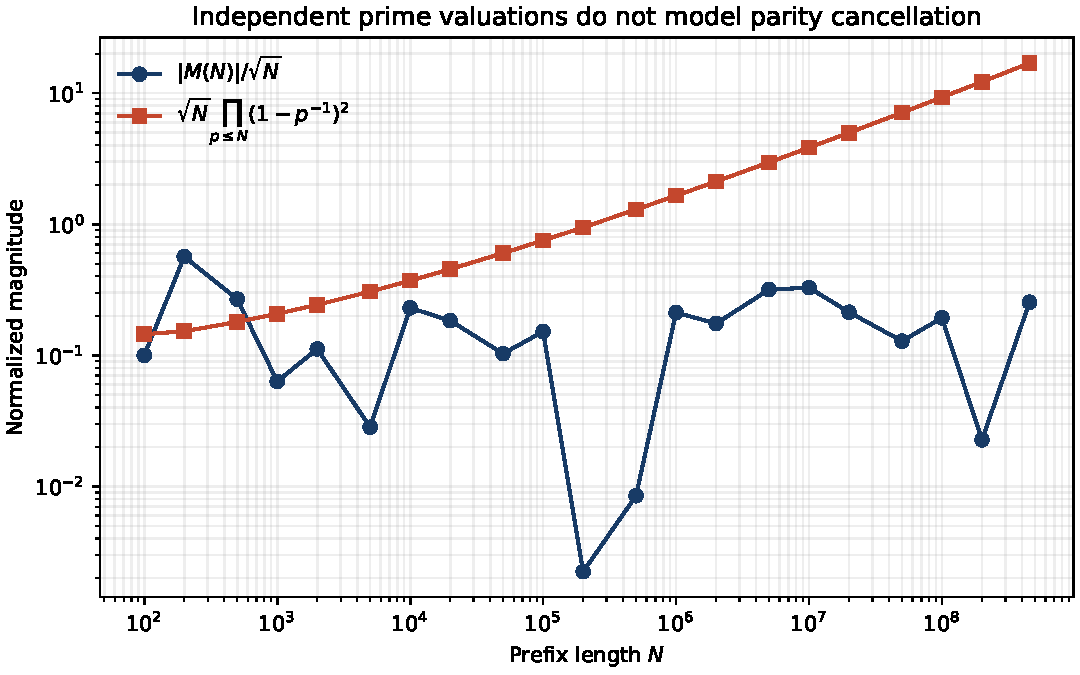
\includegraphics[width=0.88\textwidth]{boolean_product_model_mismatch.pdf}%
  }{%
    \fbox{\parbox{0.82\textwidth}{\centering
      Missing external file: \texttt{boolean\_product\_model\_mismatch.pdf}.\\
      Place it in the same directory as this \texttt{.tex} file.}}%
  }
  \caption{Reported stored M\"obius prefixes versus the mean predicted by
  the unrestricted independent \(p\)-adic surrogate.  The comparison records
  finite-scale model mismatch and is not used as evidence for an asymptotic
  pointwise theorem.}
  \label{fig:boolean-mismatch}
\end{figure}
\FloatBarrier

\section{Audit verdicts}\label{sec:verdicts}

\begin{table}[p]
\centering
\footnotesize
\caption{Uniform audit of distant square-root theories.}
\label{tab:audit}
\begin{tabularx}{\textwidth}{>{\raggedright\arraybackslash}p{0.18\textwidth}
  >{\raggedright\arraybackslash}p{0.20\textwidth}
  >{\raggedright\arraybackslash}X
  >{\raggedright\arraybackslash}p{0.15\textwidth}}
\toprule
Area & Genuine theorem & Missing interface & Audit conclusion\\
\midrule
Martingales and Stein & Square-root fluctuations and concentration for centered
random processes & Conditional centering or regression is unavailable for the
fixed M\"obius path & No applicable theorem identified\\
Boolean hypercontractivity & Sharp product-space norm inequalities & High-degree
parity and the unrestricted independent surrogate has mean
\(N/(\log N)^2\) & Surrogate mismatch; no transfer\\
Automatic sequences & Exact Rudin--Shapiro square-root recursion & Untwisting
requires a second weighted estimate; known M\"obius orthogonality is qualitative
& No square-root untwisting theorem identified\\
Frames and stable sampling & Restricted inverses, Kashin representations, paving
& The direct argument needs \(\ell^1\) control and a uniform deterministic
correlation estimate & No complete stable-transfer theorem identified\\
Discrepancy & Existence of a square-root-discrepancy coloring & The theorem chooses
the signs; M\"obius signs are prescribed & Wrong quantifier for this application\\
Transfer operators & CLT and ASIP under spectral hypotheses & Spectral gap,
centering, and deterministic control of the fixed arithmetic orbit are unproved
& No uniform fixed-orbit theorem identified\\
Empirical processes & KMT-scale approximation of centered samples & Controls
deviation from \(\Mertens(N)/N\), not that mean & Centers away the target\\
Random multiplicative chaos & Sharp moment and distribution theorems & Ambient
\(L^p\) control does not bound a prescribed phase & Deterministic-evaluation
bridge absent\\
Decoupling & Comparison of dependent and independent random chaos & Requires a
probability-space coupling and does not control a prescribed phase & No
deterministic specialization identified\\
Function fields & Exact cancellation and square-root variance theorems & No
specialization preserving intervals, M\"obius values, and constants & Solved
analogue; no transfer map\\
\bottomrule
\end{tabularx}
\end{table}
\FloatBarrier

No entry in Table~\ref{tab:audit} is admissible under
Theorem~\ref{thm:transfer}.  This statement concerns the audited theorem set;
it is not a claim that every conceivable theorem in these fields is incapable
of contributing.

\section{Closure of the conditional templates and the involution reformulation}
\label{sec:program}

\subsection{Why the two conditional templates are not retained}
\label{subsec:closed-templates}

The independent-transfer conditions used in the previous version were
necessary but not sufficient.  Requiring a theorem to hold on a class larger
than the single M\"obius instance does not create an independent proof of that
theorem.  In the frame program, the decisive input remains the uniform bound
\begin{equation}
  \sup_j\left|\langle\mu,u_j\rangle\right|
  \ll_{\eps}N^{1/2+\eps}
  \label{eq:frame-decisive-input}
\end{equation}
for a reconstructing family with substantial low-frequency content.  The
frame theorems control reconstruction norms, not the arithmetic correlations
in \eqref{eq:frame-decisive-input}.  Proposition~\ref{prop:constant-projection}
also shows that stable reconstruction prevents every normalized kernel from
being uniformly remote from the constant direction.  After the known analytic
correlation machinery has been excluded by the scope of this audit, no
independent engine remains for \eqref{eq:frame-decisive-input}.  The frame
program is therefore closed within this scope, rather than retained as a
conditional route.

The same correction applies to deterministic transfer operators.  A spectral
gap for an abstract operator gives no estimate for a prescribed arithmetic
path.  Requiring contraction for every path in a class containing the M\"obius
path would be stronger, but the proof of that contraction is precisely the
missing arithmetic input.  If it is verified through correlations of the
M\"obius path, the argument is circular; if it is not, no applicable theorem
is currently available.  Calling the class ``uniform'' or ``locally defined''
does not resolve this interface.  Thus the transfer-operator program is also
closed within the declared search.

This conclusion is scoped.  It does not prove that frame theory or dynamical
systems can never participate in a future proof.  It says that they supply no
presently independent square-root mechanism once the classical arithmetic
engines capable of proving uniform twisted estimates are removed.

\subsection{A sign-reversing involution program}
\label{subsec:involution}

Set
\begin{equation}
  \mathcal S_N=\{n\leq N:\mu(n)^2=1\},
  \qquad
  \mathcal S_N^{\pm}=\{n\in\mathcal S_N:\mu(n)=\pm1\}.
  \label{eq:squarefree-bipartition}
\end{equation}
The following elementary identity describes a different proof format:
deterministic cancellation in explicit pairs, rather than a uniform
correlation estimate.  It does not by itself make the problem easier.

\begin{proposition}[Exact cancellation by an involution]
\label{prop:involution-cancellation}
Let \(E_N\subseteq\mathcal S_N\), and let
\(T_N:\mathcal S_N\setminus E_N\to\mathcal S_N\setminus E_N\) satisfy
\begin{equation}
  T_N(T_N(n))=n,
  \qquad
  T_N(n)\neq n,
  \qquad
  \mu(T_N(n))=-\mu(n).
  \label{eq:sign-reversing-involution}
\end{equation}
Then
\begin{equation}
  \Mertens(N)=\sum_{n\in E_N}\mu(n),
  \qquad
  |\Mertens(N)|\leq |E_N|.
  \label{eq:involution-bound}
\end{equation}
\end{proposition}

\begin{proof}
Terms with \(\mu(n)=0\) do not contribute to \(\Mertens(N)\).  The involution
partitions \(\mathcal S_N\setminus E_N\) into two-element orbits.  The two
M\"obius values in each orbit sum to zero by
\eqref{eq:sign-reversing-involution}.  Only the terms in \(E_N\) remain, which
gives both assertions in \eqref{eq:involution-bound}.
\end{proof}

\subsection{What successful involutions do in other settings}
\label{subsec:successful-involutions}

There are rigorous precedents for the architecture in
Proposition~\ref{prop:involution-cancellation}.  The closest elementary
arithmetic example is
\begin{equation}
  \sum_{d\mid m}\mu(d)=0
  \qquad (m>1).
  \label{eq:divisor-cube-cancellation}
\end{equation}
After zero terms are removed, fix one prime \(p\mid m\) and toggle whether
\(p\) divides \(d\).  The squarefree divisors of \(m\) form a complete Boolean
cube, the toggle never leaves that cube, and every pair has opposite M\"obius
sign.  The interval condition \(d\leq N\) destroys precisely this closure
property when one tries to apply the same operation to \(\mathcal S_N\).

Franklin's involution for Euler's pentagonal-number theorem is a more
informative model; see Pak \cite{Pak2004}.  If \(d_e(t)\) and \(d_o(t)\) count
partitions of \(t\) into distinct parts with respectively even and odd numbers
of parts, the involution gives
\begin{equation}
  d_e(t)-d_o(t)=
  \begin{cases}
    (-1)^r,&t=r(3r-1)/2\text{ for some }r\in\mathbb Z,\\
    0,&\text{otherwise}.
  \end{cases}
  \label{eq:franklin-cancellation}
\end{equation}
Its mechanism has four components: a conserved grade \(t\), a canonical local
move, reversibility of that move, and a complete classification of the fixed
points.  Only generalized pentagonal shapes are fixed, so the number of
unpaired objects with grade at most \(X\) is \(O(\sqrt X)\).  The general
involution principle systematizes this style of cancellation
\cite{GarsiaMilne1981}.  Equation~\eqref{eq:franklin-cancellation} is therefore
a genuine example of square-root-sparse exceptions, but its conserved additive
weight and rigid normal forms have no known counterpart for products of
distinct primes.

Discrete Morse theory gives a geometric version of the same philosophy:
an acyclic matching on the face poset pairs incident cells of consecutive
dimensions, and unmatched critical cells control the resulting cell complex
\cite{Forman1998}.  The analogy is exact for Forman acyclic matchings; it is
not an identification of every sign-reversing involution with a discrete Morse
matching.  Within the Forman class it supplies a decisive obstruction.
Define
\begin{equation}
  \Delta_N=\{P(n):n\leq N\text{ is squarefree}\},
  \qquad
  P(n)=\{p:p\mid n\}.
  \label{eq:bjorner-complex}
\end{equation}
This is a simplicial complex because divisors of a squarefree integer not
exceeding \(N\) also do not exceed \(N\).  Bj\"orner proved
\begin{equation}
  \Mertens(N)=-\widetilde\chi(\Delta_N)
  =\sum_{k\geq0}(-1)^{k-1}\beta_k(\Delta_N),
  \label{eq:mertens-euler-characteristic}
\end{equation}
and, for every \(\theta>17/54\),
\begin{equation}
\begin{aligned}
  \sum_{k\geq0}\beta_k(\Delta_N)
    &=\frac{2N}{\pi^2}+O_{\theta}(N^{\theta}),\\
  \sum_{k\equiv 0 \pmod 2}\beta_k(\Delta_N)
    &\sim
    \sum_{k\equiv 1 \pmod 2}\beta_k(\Delta_N)
    \sim\frac{N}{\pi^2}.
\end{aligned}
  \label{eq:bjorner-betti-mass}
\end{equation}
See \cite{Bjorner2011}.  By the weak Morse inequalities, every Forman discrete
Morse function on \(\Delta_N\) has at least \(\beta_k(\Delta_N)\) critical
\(k\)-cells.  Hence its total number of critical cells is bounded below by a
positive constant times \(N\), not by \(N^{1/2+\eps}\).  Standard discrete
Morse matching therefore cannot supply the desired sparse exceptional set.
The cancellation in \eqref{eq:mertens-euler-characteristic} occurs between two
quantities of linear size and is exactly the unresolved arithmetic
cancellation.  Thus the Euler-characteristic formulation is an established
translation, not a new route to the target.

An odd-block involution would not be a Forman matching: it may replace several
vertices at once and need not pair incident faces.  This departure is necessary
to escape \eqref{eq:bjorner-betti-mass}, but it also forfeits the Morse-theoretic
machinery that proves cancellation and controls critical cells in other
complexes.

The simplest multiplicative graph cannot achieve the target.  Let \(G_N^{(1)}\)
have vertex set \(\mathcal S_N\), with an edge between \(n\) and \(pn\) whenever
\(p\) is prime, \(p\nmid n\), and \(pn\leq N\).  Every edge reverses the
M\"obius sign.

\begin{proposition}[Large-prime obstruction to one-prime pairing]
\label{prop:one-prime-obstruction}
Every matching in \(G_N^{(1)}\) leaves at least
\begin{equation}
  \pi(N)-\pi(N/2)-1
  \label{eq:large-prime-unmatched}
\end{equation}
vertices unmatched.  Consequently, one-prime involutions have an exceptional
set bounded below by a positive constant multiple of \(N/\log N\) for all
sufficiently large \(N\).
\end{proposition}

\begin{proof}
If \(\ell\) is prime and \(N/2<\ell\leq N\), then \(\ell\) cannot be multiplied
by any prime while remaining at most \(N\).  If \(\ell=pn\) with \(p\) prime,
then primality forces \(n=1\).  Thus every such \(\ell\) has the unique neighbor
\(1\) in \(G_N^{(1)}\).  A matching can pair at most one of these primes with
\(1\), proving \eqref{eq:large-prime-unmatched}.  The prime number theorem gives
the final order statement \cite{MontgomeryVaughan2007}.
\end{proof}

This obstruction is consistent with the appearance of the scale
\(N/\log N\) in the ordinary divisor graph; see Melotti and Saias
\cite{MelottiSaias2020}.  It forces any surviving involution to use more than
single-prime divisibility edges.

\begin{definition}[Odd-block multiplicative move]
\label{def:odd-block-move}
For \(n,m\in\mathcal S_N\), write \(P(n)\) for the set of prime divisors of
\(n\).  An odd-block move from \(n\) to \(m\) is a replacement
\begin{equation}
\begin{aligned}
  m&=n\frac{\prod_{p\in A}p}{\prod_{q\in B}q},
  & A\cap P(n)&=\varnothing,\\
  B&\subseteq P(n),
  & |A|+|B|&\equiv1\pmod 2.
\end{aligned}
  \label{eq:odd-block-move}
\end{equation}
It is multiplicatively \(C\)-balanced when
\begin{equation}
  C^{-1}\leq
  \frac{\prod_{p\in A}p}{\prod_{q\in B}q}
  \leq C.
  \label{eq:block-balance}
\end{equation}
\end{definition}

The parity condition in \eqref{eq:odd-block-move} gives
\(\mu(m)=-\mu(n)\).  In particular, a large prime may be paired with a product
of two smaller primes by replacing one prime with two, a three-coordinate
change that is unavailable in \(G_N^{(1)}\).

The unproved search target is an explicit involution made from balanced
odd-block moves for which, for every \(\eps>0\),
\begin{equation}
  |E_N|\ll_{\eps}N^{1/2+\eps}.
  \label{eq:odd-block-target}
\end{equation}
Proposition~\ref{prop:involution-cancellation} would then give
\eqref{eq:target} immediately.  Equation~\eqref{eq:odd-block-target} is not
proved here.

The construction is noncircular only if the pairing rule is specified from
prime supports and fixed scale partitions before \(\Mertens(N)\) is evaluated,
its injectivity is proved directly, and its exceptional set is counted through
unsigned factorization conditions.  Merely computing a maximum matching, or
invoking Hall's theorem \cite{Hall1935} without proving its neighborhood
inequalities independently of the sign imbalance, relocates the original
problem.  Indeed, \eqref{eq:involution-bound} implies the unavoidable lower
bound \(|E_N|\geq|\Mertens(N)|\) for every sign-reversing partial involution.
The only possible new content would therefore be an explicit multiscale
pairing whose exceptional set can be bounded using only the geometry of prime
factorizations.  No such square-root construction, partial exponent improving
the one-prime barrier, or theorem suggesting that it exists is presently
supplied.  More importantly, any estimate \(|E_N|\leq B(N)\) for a
sign-reversing involution immediately gives
\(|\Mertens(N)|\leq B(N)\) by
Proposition~\ref{prop:involution-cancellation}.  The exceptional-set theorem
is therefore not an intermediate transfer theorem: it is a direct sufficient
condition for the corresponding Mertens bound.

An earlier version proposed \(o(N/\log N)\) as a first exceptional-set target.
That target is withdrawn because it is weaker than the known unconditional
estimate
\begin{equation}
  \Mertens(N)\ll
  N\exp\!\left\{-c(\log N)^{3/5}(\log\log N)^{-1/5}\right\}
  \qquad(N\geq N_0),
  \label{eq:known-mertens-bound}
\end{equation}
for suitable constants \(c>0\) and \(N_0\); explicit versions are given by
Lee and Leong \cite{LeeLeong2024}.  A fixed-power exceptional-set estimate
\(|E_N|\ll N^{1-\delta}\) would instead constitute a major new pointwise
bound for \(\Mertens(N)\) through the same elementary identity.  It cannot be
advertised as a modest preliminary objective.

The parity of the number of prime factors is precisely the information hidden
by the classical sieve parity phenomenon.  Friedlander and Iwaniec's
asymptotic sieve overcomes that phenomenon in special sequences by adding
bilinear information \cite{FriedlanderIwaniec1998}.  If an exceptional-set
estimate requires such parity-sensitive cancellation, the proposed
combinatorial language has returned to the analytic machinery excluded from
this audit.  The odd-block proposal is therefore closed as a forward program,
while its exact formulation remains in the report as a record of the
obstruction.

Automatic paraunitary recursions are removed from the forward program.  Their
exact square-root mechanism controls the recursively generated automatic
sequence itself, while Proposition~\ref{prop:untwist} shows that inserting and
then removing an automatic weight requires a second uncontrolled correlation.
M\"ullner's qualitative orthogonality theorem supplies no missing stable
inverse or second-channel estimate.  This does not constitute an impossibility
theorem, but it leaves no noncircular transfer mechanism to pursue.

Function-field comparison is also removed.  The exact analogues remain useful
as controls, but no candidate specialization currently preserves the interval,
the M\"obius values, and subpolynomial constants.  Without a proposed normed
map, the analogy does not define a research route that can be audited by
Theorem~\ref{thm:transfer}.

\section{Conclusion}\label{sec:conclusion}

The audit found many exact square-root theorems far from classical analytic
number theory, but no existing theorem that can presently be transferred to
\(\Mertens(N)\) at square-root scale.  The failure mechanisms are now explicit:
unknown centering for martingales and empirical processes, high-degree parity
misrepresented by product probability, untwisting for automatic sequences,
\(\ell^1\) loss in the direct frame argument, choice of signs in discrepancy,
exceptional fixed orbits for transfer operators, absence of an ambient-to-point
estimate for random chaos, and absence of a normed specialization from function
fields.

The exact-transfer lemma remains a strict diagnostic for future transference
candidates.  It does not, however, manufacture the decisive uniform
correlation estimate.  The earlier decision to retain signed frames and
uniform deterministic operators mistook a well-posed missing hypothesis for an
independent mechanism.  Both are now closed within the deliberately distant
scope of this audit.  Automatic recursions and function-field analogy likewise
remain only as negative controls.

No forward route in the audited collection survives under the declared
exclusions.  The sign-reversing-involution section
does not alter that verdict.  Proposition~\ref{prop:one-prime-obstruction}
proves that its naive local version leaves order \(N/\log N\) vertices
unmatched, while Proposition~\ref{prop:involution-cancellation} shows that any
exceptional-set estimate immediately implies the corresponding pointwise
Mertens bound.  The previously proposed \(o(N/\log N)\) milestone has been
removed because it is weaker than the unconditional estimate
\eqref{eq:known-mertens-bound}.

Nor does cyclic-window energy provide a bridge.  The exact decomposition in
Proposition~\ref{prop:window-energy} shows that the uncentered energy already
contains the desired constant mode as a nonnegative orthogonal component;
centering removes that component rather than estimating it.  Thus the
window argument is another exact reformulation, not a source of cancellation.
Within the audited collection, no completed transfer route or independently
proved intermediate estimate remains.  This scoped conclusion is not an
impossibility theorem for
future mathematics outside that collection.

\begin{thebibliography}{99}

\bibitem{Beckner1975}
W. Beckner,
\emph{Inequalities in Fourier analysis},
Ann. of Math. (2) \textbf{102} (1975), 159--182.
\href{https://doi.org/10.2307/1970980}{doi:10.2307/1970980}.

\bibitem{Bonami1970}
A. Bonami,
\emph{\'Etude des coefficients de Fourier des fonctions de \(L^p(G)\)},
Ann. Inst. Fourier (Grenoble) \textbf{20} (1970), no.~2, 335--402.
\href{https://doi.org/10.5802/aif.357}{doi:10.5802/aif.357}.

\bibitem{Bjorner2011}
A. Bj\"orner,
\emph{A cell complex in number theory},
Adv. Appl. Math. \textbf{46} (2011), no.~1--4, 71--85.
\href{https://doi.org/10.1016/j.aam.2010.09.007}%
{doi:10.1016/j.aam.2010.09.007}.

\bibitem{Chatterjee2007}
S. Chatterjee,
\emph{Stein's method for concentration inequalities},
Probab. Theory Related Fields \textbf{138} (2007), 305--321.
\href{https://doi.org/10.1007/s00440-006-0029-y}{doi:10.1007/s00440-006-0029-y}.

\bibitem{deLaPenaGine1999}
V. H. de la Pe\~na and E. Gin\'e,
\emph{Decoupling: From Dependence to Independence},
Probability and its Applications, Springer, New York, 1999.
\href{https://doi.org/10.1007/978-1-4612-0537-1}{doi:10.1007/978-1-4612-0537-1}.

\bibitem{Gordin1969}
M. I. Gordin,
\emph{The central limit theorem for stationary processes},
Dokl. Akad. Nauk SSSR \textbf{188} (1969), 739--741.
\url{https://www.mathnet.ru/eng/dan34921}.

\bibitem{Forman1998}
R. Forman,
\emph{Morse theory for cell complexes},
Adv. Math. \textbf{134} (1998), no.~1, 90--145.
\href{https://doi.org/10.1006/aima.1997.1650}%
{doi:10.1006/aima.1997.1650}.

\bibitem{FriedlanderIwaniec1998}
J. Friedlander and H. Iwaniec,
\emph{Asymptotic sieve for primes},
Ann. of Math. (2) \textbf{148} (1998), no.~3, 1041--1065.
\href{https://doi.org/10.2307/121035}{doi:10.2307/121035}.

\bibitem{GarsiaMilne1981}
A. M. Garsia and S. C. Milne,
\emph{A Rogers--Ramanujan bijection},
J. Combin. Theory Ser. A \textbf{31} (1981), no.~3, 289--339.
\href{https://doi.org/10.1016/0097-3165(81)90062-5}%
{doi:10.1016/0097-3165(81)90062-5}.

\bibitem{GordinPeligrad2011}
M. Gordin and M. Peligrad,
\emph{On the functional central limit theorem via martingale approximation},
Bernoulli \textbf{17} (2011), 424--440.
\href{https://doi.org/10.3150/10-BEJ276}{doi:10.3150/10-BEJ276}.

\bibitem{Gouezel2010}
S. Gou\"ezel,
\emph{Almost sure invariance principle for dynamical systems by spectral
methods},
Ann. Probab. \textbf{38} (2010), 1639--1671.
\href{https://doi.org/10.1214/10-AOP525}{doi:10.1214/10-AOP525}.

\bibitem{Harper2020}
A. J. Harper,
\emph{Moments of random multiplicative functions, I: Low moments, better than
square-root cancellation, and critical multiplicative chaos},
Forum Math. Pi \textbf{8} (2020), e1.
\href{https://doi.org/10.1017/fmp.2019.7}{doi:10.1017/fmp.2019.7}.

\bibitem{KeatingRudnick2016}
J. P. Keating and Z. Rudnick,
\emph{Squarefree polynomials and M\"obius values in short intervals and
arithmetic progressions},
Algebra Number Theory \textbf{10} (2016), 375--420.
\href{https://doi.org/10.2140/ant.2016.10.375}{doi:10.2140/ant.2016.10.375}.

\bibitem{KMT1975}
J. Koml\'os, P. Major, and G. Tusn\'ady,
\emph{An approximation of partial sums of independent random variables, and
the sample distribution function. I},
Z. Wahrscheinlichkeitstheorie verw. Gebiete \textbf{32} (1975), 111--131.
\href{https://doi.org/10.1007/BF00533093}{doi:10.1007/BF00533093}.

\bibitem{LeeLeong2024}
E. S. Lee and N. Leong,
\emph{New explicit bounds for the Mertens function and the reciprocal of the
Riemann zeta-function},
preprint, revised 2024.
\href{https://arxiv.org/abs/2208.06141}{arXiv:2208.06141}.

\bibitem{LyubarskiiVershynin2010}
Y. Lyubarskii and R. Vershynin,
\emph{Uncertainty principles and vector quantization},
IEEE Trans. Inform. Theory \textbf{56} (2010), 3491--3501.
\href{https://doi.org/10.1109/TIT.2010.2048458}{doi:10.1109/TIT.2010.2048458}.

\bibitem{MontgomeryVaughan2007}
H. L. Montgomery and R. C. Vaughan,
\emph{Multiplicative Number Theory I: Classical Theory},
Cambridge Studies in Advanced Mathematics, vol.~97,
Cambridge University Press, Cambridge, 2007.
\href{https://doi.org/10.1017/CBO9780511618314}%
{doi:10.1017/CBO9780511618314}.

\bibitem{MSS2015}
A. W. Marcus, D. A. Spielman, and N. Srivastava,
\emph{Interlacing families II: Mixed characteristic polynomials and the
Kadison--Singer problem},
Ann. of Math. (2) \textbf{182} (2015), 327--350.
\href{https://doi.org/10.4007/annals.2015.182.1.8}{doi:10.4007/annals.2015.182.1.8}.

\bibitem{Muellner2017}
C. M\"ullner,
\emph{Automatic sequences fulfill the Sarnak conjecture},
Duke Math. J. \textbf{166} (2017), 3219--3290.
\href{https://doi.org/10.1215/00127094-2017-0024}{doi:10.1215/00127094-2017-0024}.

\bibitem{NaorYoussef2017}
A. Naor and P. Youssef,
\emph{Restricted invertibility revisited},
in \emph{A Journey Through Discrete Mathematics}, Springer, Cham, 2017,
657--691.
\href{https://doi.org/10.1007/978-3-319-44479-6_27}%
{doi:10.1007/978-3-319-44479-6\_27}.

\bibitem{Hall1935}
P. Hall,
\emph{On representatives of subsets},
J. London Math. Soc. \textbf{s1-10} (1935), no.~1, 26--30.
\href{https://doi.org/10.1112/jlms/s1-10.37.26}%
{doi:10.1112/jlms/s1-10.37.26}.

\bibitem{MelottiSaias2020}
P. Melotti and E. Saias,
\emph{On path partitions of the divisor graph},
Acta Arith. \textbf{192} (2020), no.~4, 329--339.
\href{https://doi.org/10.4064/aa180711-26-4}%
{doi:10.4064/aa180711-26-4}.

\bibitem{PeligradUtev2005}
M. Peligrad and S. Utev,
\emph{A new maximal inequality and invariance principle for stationary
sequences},
Ann. Probab. \textbf{33} (2005), 798--815.
\href{https://doi.org/10.1214/009117904000001035}{doi:10.1214/009117904000001035}.

\bibitem{Pak2004}
I. Pak,
\emph{The nature of partition bijections I: Involutions},
Adv. Appl. Math. \textbf{33} (2004), no.~2, 263--289.
\href{https://doi.org/10.1016/j.aam.2003.08.007}%
{doi:10.1016/j.aam.2003.08.007}.

\bibitem{Rudin1959}
W. Rudin,
\emph{Some theorems on Fourier coefficients},
Proc. Amer. Math. Soc. \textbf{10} (1959), 855--859.
\href{https://doi.org/10.1090/S0002-9939-1959-0116184-5}{doi:10.1090/S0002-9939-1959-0116184-5}.

\bibitem{SoundXu2023}
K. Soundararajan and M. W. Xu,
\emph{Central limit theorems for random multiplicative functions},
J. Anal. Math. \textbf{151} (2023), 343--374.
\href{https://doi.org/10.1007/s11854-023-0331-y}{doi:10.1007/s11854-023-0331-y}.

\bibitem{Spencer1985}
J. Spencer,
\emph{Six standard deviations suffice},
Trans. Amer. Math. Soc. \textbf{289} (1985), 679--706.
\href{https://doi.org/10.2307/2000258}{doi:10.2307/2000258}.

\end{thebibliography}

\end{document}
